\documentclass[10pt]{beamer}
\usetheme[
%%% option passed to the outer theme
%    progressstyle=fixedCircCnt,   % fixedCircCnt, movingCircCnt (moving is deault)
]{Feather}
  
% If you want to change the colors of the various elements in the theme, edit and uncomment the following lines

% Change the bar colors:
%\setbeamercolor{Feather}{fg=red!20,bg=red}

% Change the color of the structural elements:
%\setbeamercolor{structure}{fg=red}

% Change the frame title text color:
%\setbeamercolor{frametitle}{fg=blue}

% Change the normal text color background:
%\setbeamercolor{normal text}{fg=black,bg=gray!10}

%-------------------------------------------------------
% INCLUDE PACKAGES
%-------------------------------------------------------

\usepackage[utf8]{inputenc}
\usepackage[italian]{babel}
\usepackage{helvet}
\usepackage{listings}
\usepackage{xcolor}
\usepackage{graphicx}

%-------------------------------------------------------
% DEFFINING AND REDEFINING COMMANDS
%-------------------------------------------------------

% colored hyperlinks
\newcommand{\chref}[2]{
  \href{#1}{{\usebeamercolor[bg]{Feather}#2}}
}

%-------------------------------------------------------
% INFORMATION IN THE TITLE PAGE
%-------------------------------------------------------

\title[Performance Modeling of Computer Systems and Networks] % [] is optional - is placed on the bottom of the sidebar on every slide
{ % is placed on the title page
      \textbf{Performance Modeling of Computer Systems and Networks}
}

\subtitle[ - Project 2018-2019]
{
      \textbf{Project 2018-2019}
}

\author[Andrea Graziani - 0273395]
{      Andrea Graziani - 0273395 \\
      {}
}

\institute[]
{
      Universit`a degli Studi di Roma “Tor Vergata” \\
      FACOLTA' DI INGEGNERIA \\
      Corso di Laurea Magistrale in Ingegneria Informatica
  
  %there must be an empty line above this line - otherwise some unwanted space is added between the university and the country (I do not know why;( )
}

\date{\today}

% ----------------------------------------------------------------------------------------- %
% Usato per personalizzare l'ambiente 'listings'...
% ----------------------------------------------------------------------------------------- %
\lstset{
language=C,
basicstyle=\tiny\ttfamily,			
keywordstyle=\color{blue},
commentstyle=\color{gray},			
stringstyle=\color{black},			
numbers=left,						
numberstyle=\tiny,					
stepnumber=1,						
breaklines=true						
}

%-------------------------------------------------------
% THE BODY OF THE PRESENTATION
%-------------------------------------------------------

\begin{document}

%-------------------------------------------------------
% THE TITLEPAGE
%-------------------------------------------------------

{\1% % this is the name of the PDF file for the background
\begin{frame}[plain,noframenumbering] % the plain option removes the header from the title page, noframenumbering removes the numbering of this frame only
  \titlepage % call the title page information from above
\end{frame}}




\section{Statistics Results}

% ----------------------------------------------------------------------------------------- %
\begin{frame}[fragile]{Statistics Results}{Il processo client}

\vspace*{20px}
Do \textbf{steady-state} statistics exist?


\end{frame}

\begin{frame}[fragile]{Statistics Results}{Il processo client}
\begin{figure}
\centering
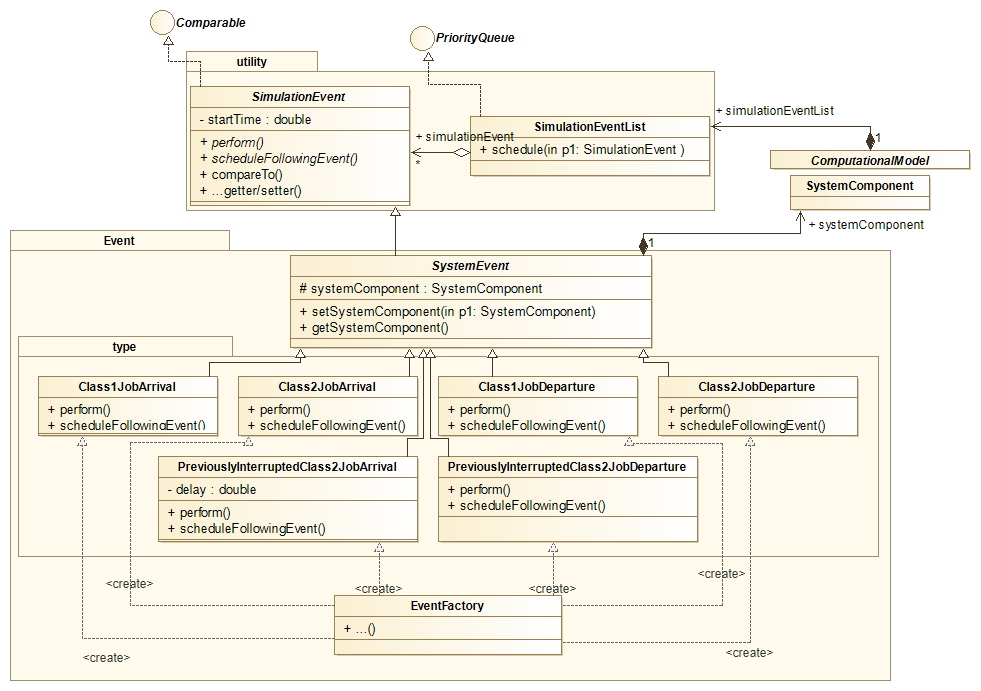
\includegraphics[width=\textwidth]{./images/ClassDiagramEvent.png}
\caption{Class 1 Jobs Service Time}
\label{fig:Concorrente}
\end{figure}


\end{frame}


% ----------------------------------------------------------------------------------------- %
\begin{frame}[fragile]{Statistics Results}{Il processo client}

\begin{block}{Steady-state system statistics}
\textbf{Steady-state system statistics} are those statistics, if they exist, that are produced by simulating the operation of a \textbf{stationary} discrete-event system for an effectively \textbf{infinite} length of time.

In many systems, a steady state is not achieved until some time after the system is started or initiated. This initial situation is often identified as a transient state, start-up or warm-up period.

If a system is in a steady state, then the recently observed behavior of the system will continue into the future.

if the variables (called state variables) which define the behavior of the system or the process are unchanging in time.

\end{block}
\end{frame}

% ----------------------------------------------------------------------------------------- %
\begin{frame}[fragile]{Statistics Results}{}

\begin{figure}
\centering
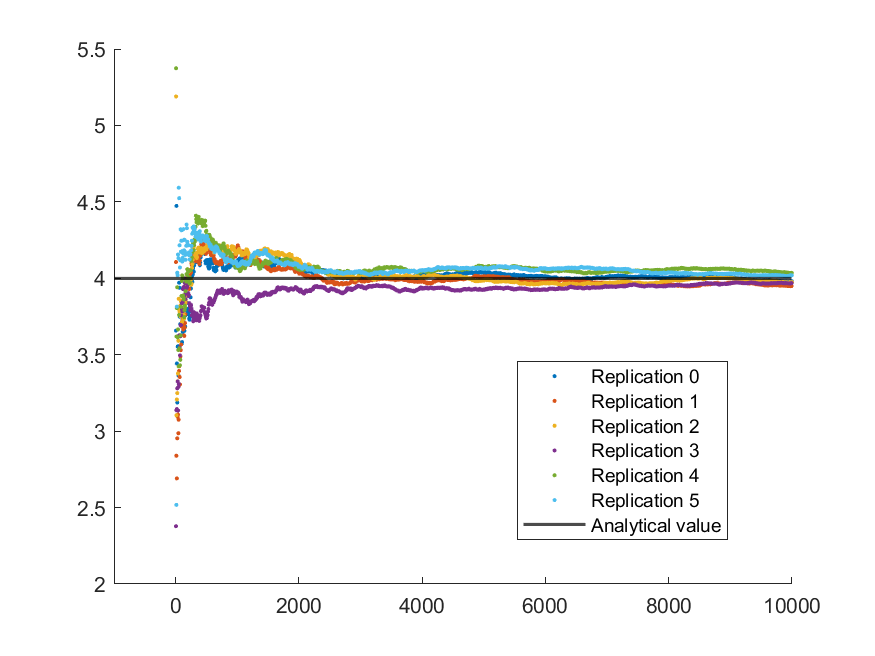
\includegraphics[width=\textwidth]{./images/ScatterPlotCloud_Class1JobsServiceTime.png}
\caption{Class 1 Jobs Service Time}
\label{fig:Concorrente}
\end{figure}


\end{frame}






% ----------------------------------------------------------------------------------------- %
\subsection{Il processo client 2}
\begin{frame}[fragile]{Architettura dell'applicazione}{Il processo client}
% ----------------------------------------------------------------------------------------- %

Analizzando la funzione \texttt{client\_start} è facile intuire che l'invio di un messaggio di richiesta e dunque l'inizio di una trasmissione prevede:

\begin{itemize}
\item L'inizializzazione di una struttura dati denominata \texttt{RequestPacket}.
\item L'invio della suddetta struttura al server attraverso l'ausilio di una struttura di tipo \texttt{DataNetwork}.
\item Attesa della risposta dal server; in caso di mancata risposta occorre rinviare un nuovo messaggio di richiesta.
\end{itemize}



\end{frame}



% ----------------------------------------------------------------------------------------- %
\subsection{Il processo client 3}
\begin{frame}[fragile]{Architettura dell'applicazione}{Il processo client}
% ----------------------------------------------------------------------------------------- %

\begin{block}{La struttura dati \texttt{DataNetwork}}
Una struttura dati di tipo \texttt{DataNetwork} rappresenta tecnicamente un contenitore per tutte le informazioni necessarie per comunicare con un host tra cui l'\textbf{indirizzo IP} e il \textbf{numero di porta}. 
\end{block}

\begin{lstlisting}[frame=lines, caption={Implementazione della struttura \texttt{DataNetwork}}]
typedef struct data_network {

	/* Socket file descriptor */
	int socket_fd;
	/* Internet socket address */
	struct sockaddr_in address;
	/* Internet socket address length */
	socklen_t address_len;

} DataNetwork;

\end{lstlisting}
\end{frame}

% ----------------------------------------------------------------------------------------- %
\subsection{Il processo client 4}
\begin{frame}[fragile]{Architettura dell'applicazione}{Il processo client}
% ----------------------------------------------------------------------------------------- %

\begin{block}{Problema}
Il server UDP deve poter scambiare più di un pacchetto con il client per poter soddisfarne le richieste. Il problema è che \textbf{l'unico numero di porta noto} al client per poter comunicare con il server è, sfortunatamente, \textbf{la stessa porta utilizzata da quest'ultimo per ricevere nuove richieste}.
\end{block}

\end{frame}

% ----------------------------------------------------------------------------------------- %
\subsection{Il processo client 5}
\begin{frame}[fragile]{Architettura dell'applicazione}{Il processo client}
% ----------------------------------------------------------------------------------------- %

\begin{block}{Soluzione}
I thread incaricati di soddisfare le richieste hanno il compito di \textbf{creare un'apposita socket di supporto} eseguendo il \textbf{binding su una porta effimera} e utilizzando quel socket per inviare e ricevere i successivi messaggi con un client.
\end{block}

\vspace*{10px}
Il client deve guardare \textbf{il numero di porta della prima risposta del server} e dunque inviare i pacchetti successivi a quella porta. \\

\vspace*{10px}
Da un punto di vista implementativo ciò è reso possibile dalla funzione \texttt{\_\_receive\_datagram} la quale provvede ad \textbf{aggiornare il contenuto della struttura \texttt{DataNetwork}} dopo la ricezione della prima risposta. Tutto ciò permette al client di \textbf{ignorare tutti quei pacchetti non provenienti dal processo server con cui interagisce}.
\end{frame}



% ----------------------------------------------------------------------------------------- %
\subsection{Schema di funzionamento}
\begin{frame}{Architettura dell'applicazione}{Schema di funzionamento}
% ----------------------------------------------------------------------------------------- %


%\begin{figure}
%\centering
%\includegraphics[width=\textwidth]{Concorrente}
%\caption{Schema del funzionamento di un server concorrente.}
%\label{fig:Concorrente}
%\end{figure}

\end{frame}








{\1
\begin{frame}[plain,noframenumbering]
  \finalpage{Grazie per l'attenzione!}
\end{frame}}


\end{document}